\documentclass[11pt]{article}
\usepackage[tmargin=1in,bmargin=1in,lmargin=1in,rmargin=1in]{geometry}
\renewcommand{\baselinestretch}{1.1} 
\usepackage{parskip}
%just so its in one place
\begin{document}

\section{Good stuff for pressure sensor}
Wearable device,\\
fits basically all body types\\
(show psych research), some evidence it works\\
small, fits portability requirement, somewhat lightweight\\
not super duper complex, so durability isnt that bad\\
really hard for the thing to *not* work, will need heavy user misuse\\
i am typing 
\section{Limitations and weaknesses for pressure sensor} %VERY IMPORTANT!!!!!!!!!!!! (see IAT)
Scope limited to backed chairs, although many (most?) chairs in Uoft (at least the engineering/physSci area) are backed. \\
electronic, can have intereference with pacemakers and stuff (goes against goal of adressing all engscis. also electricity introduces complexity which can be dangerous.\\
survey said people are aware of bad posture, so like the app/notificaiton part will need a lot of primary research to see if it works
\section{design decisions for pressure sensor DESIGN (not prototype)}
used easily accesibly pressure sensor (originally designed for robo)\\
(need to acc specify but) placed at some location so it detects pressure
testing showed that that location was pretty high up\\
wearable to an extent, lightweight so it can be worn all day sorta thing\\
easy to connect to *some notification thing which we need to specify*, which is accesible to many engscis.\\
need a couple more...
ALL ABOUT PILLOWk

\begin{figure}
    \centering
    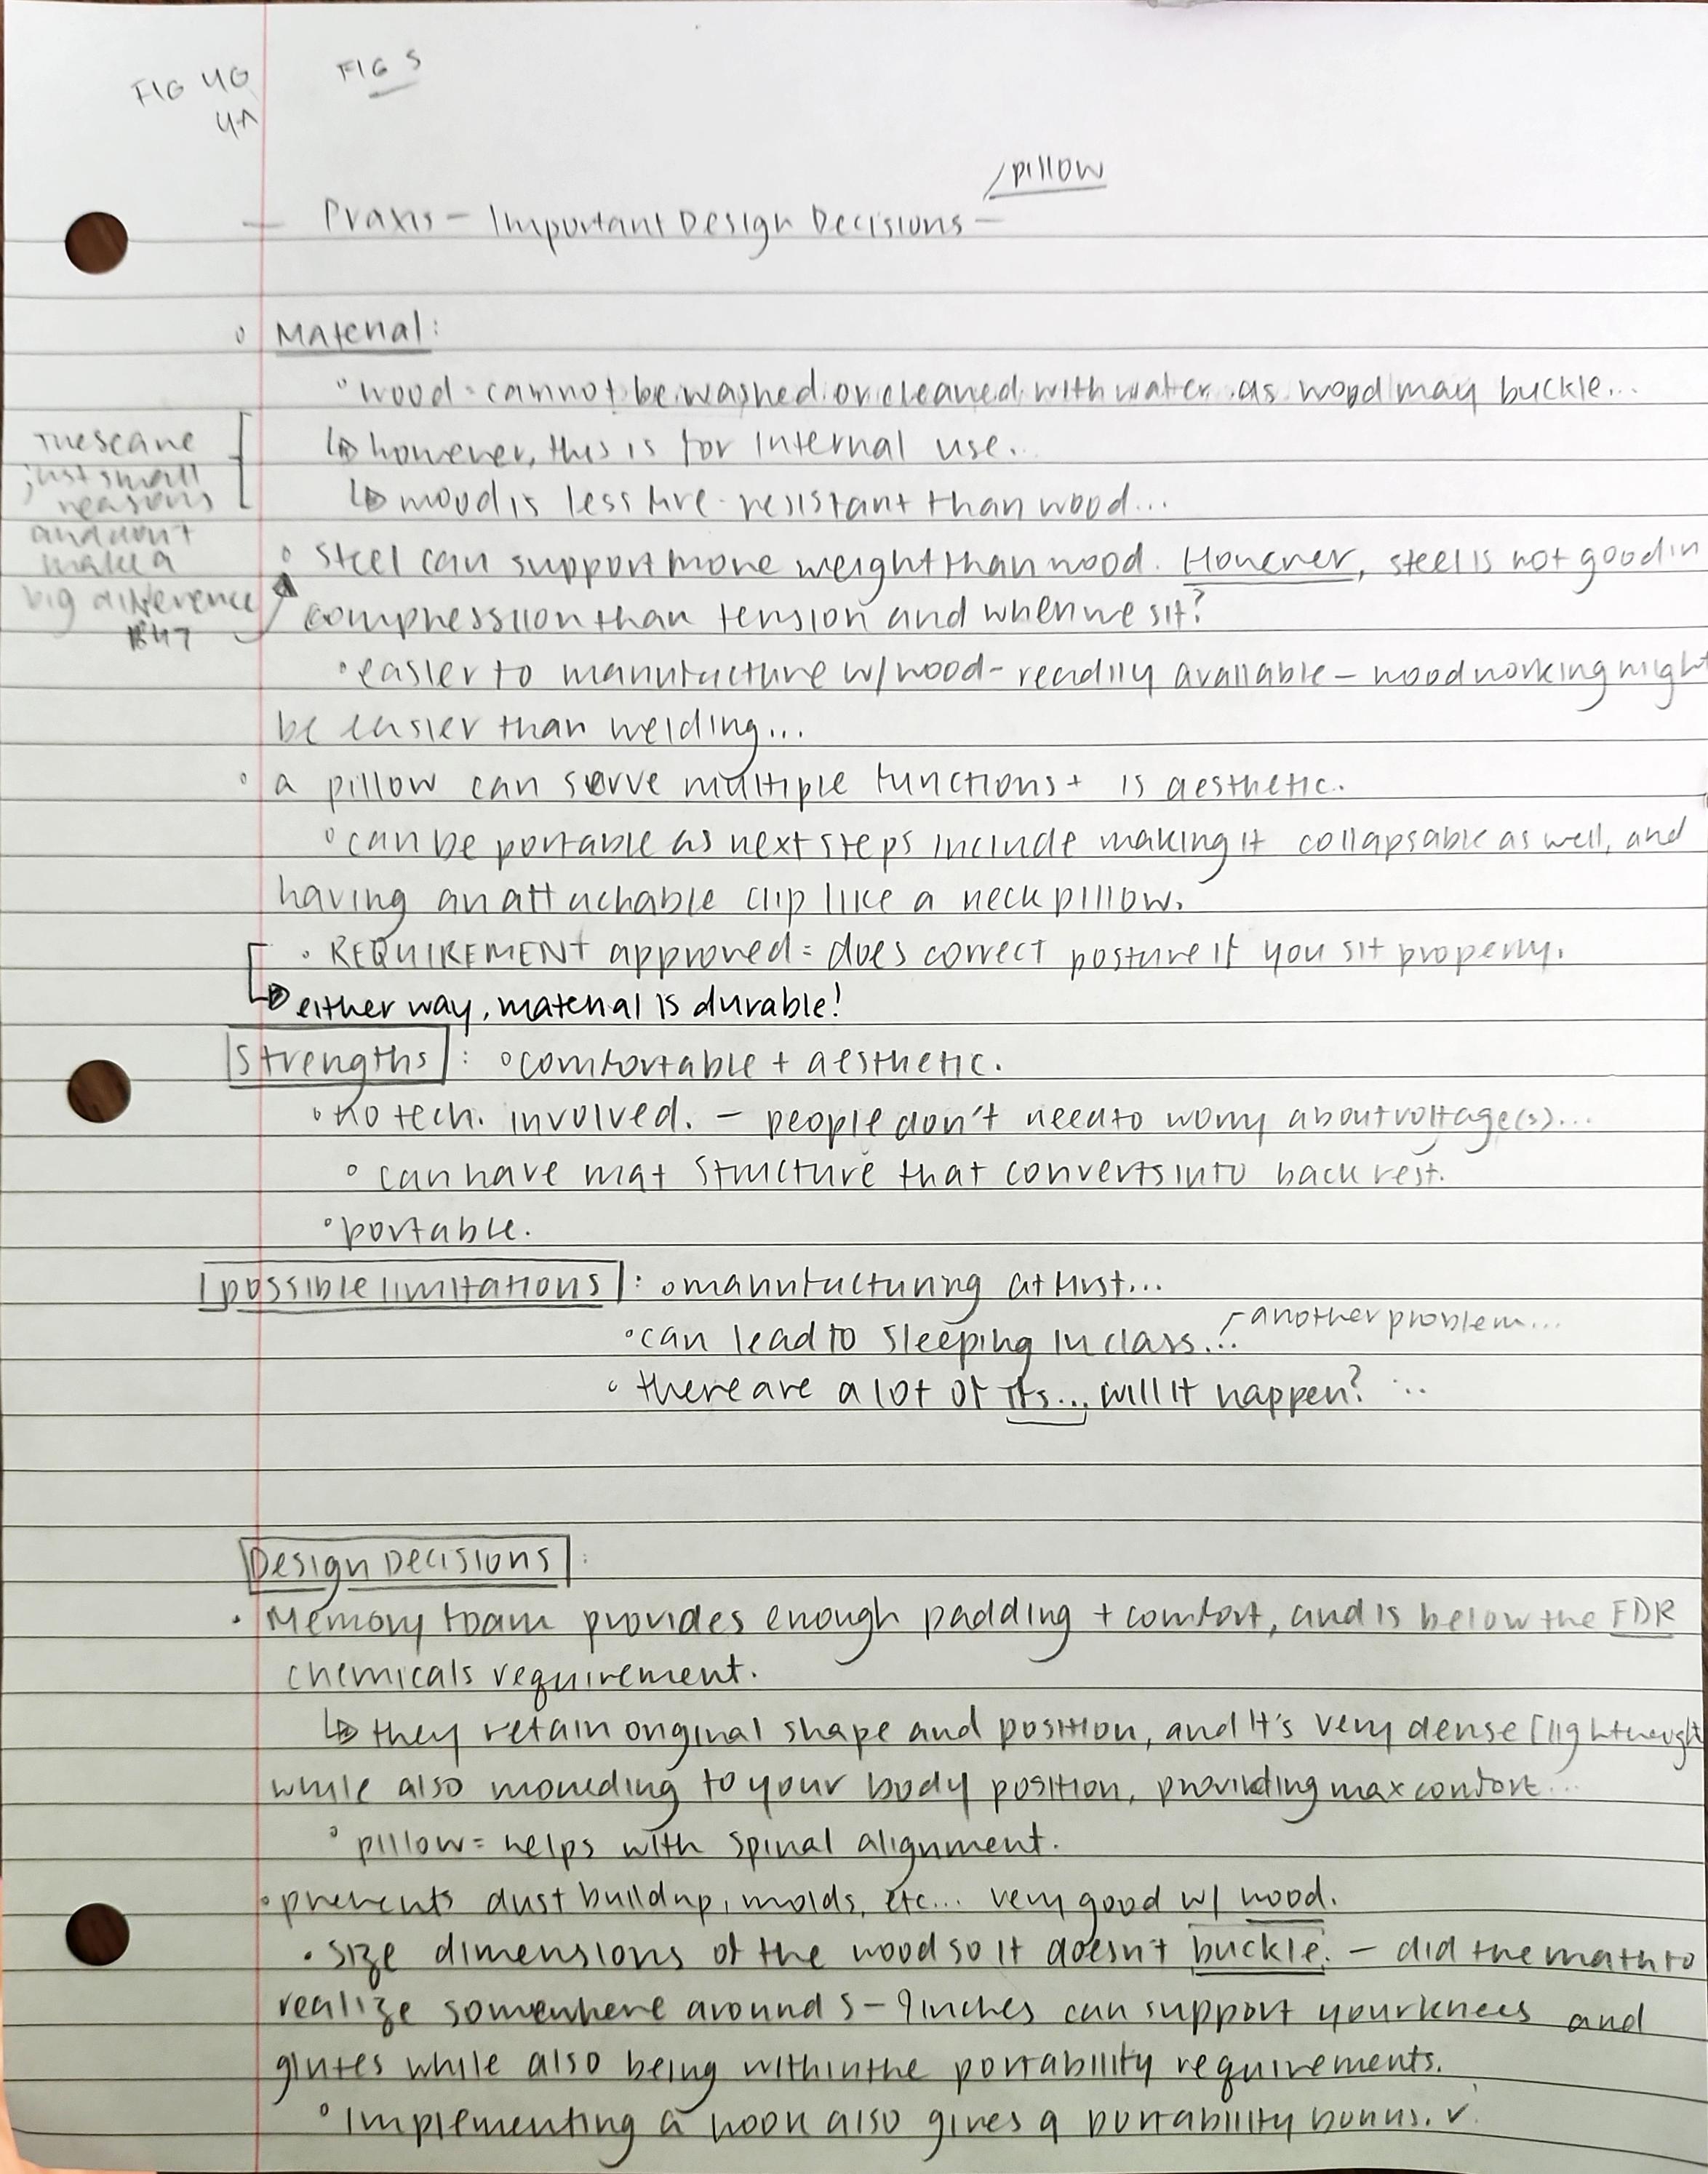
\includegraphics[width=1\linewidth]{pro-0jBrI1RE.jpeg}
    \caption{Enter Caption}
    \label{fig:enter-label}
\begin{figure}
    \centering
    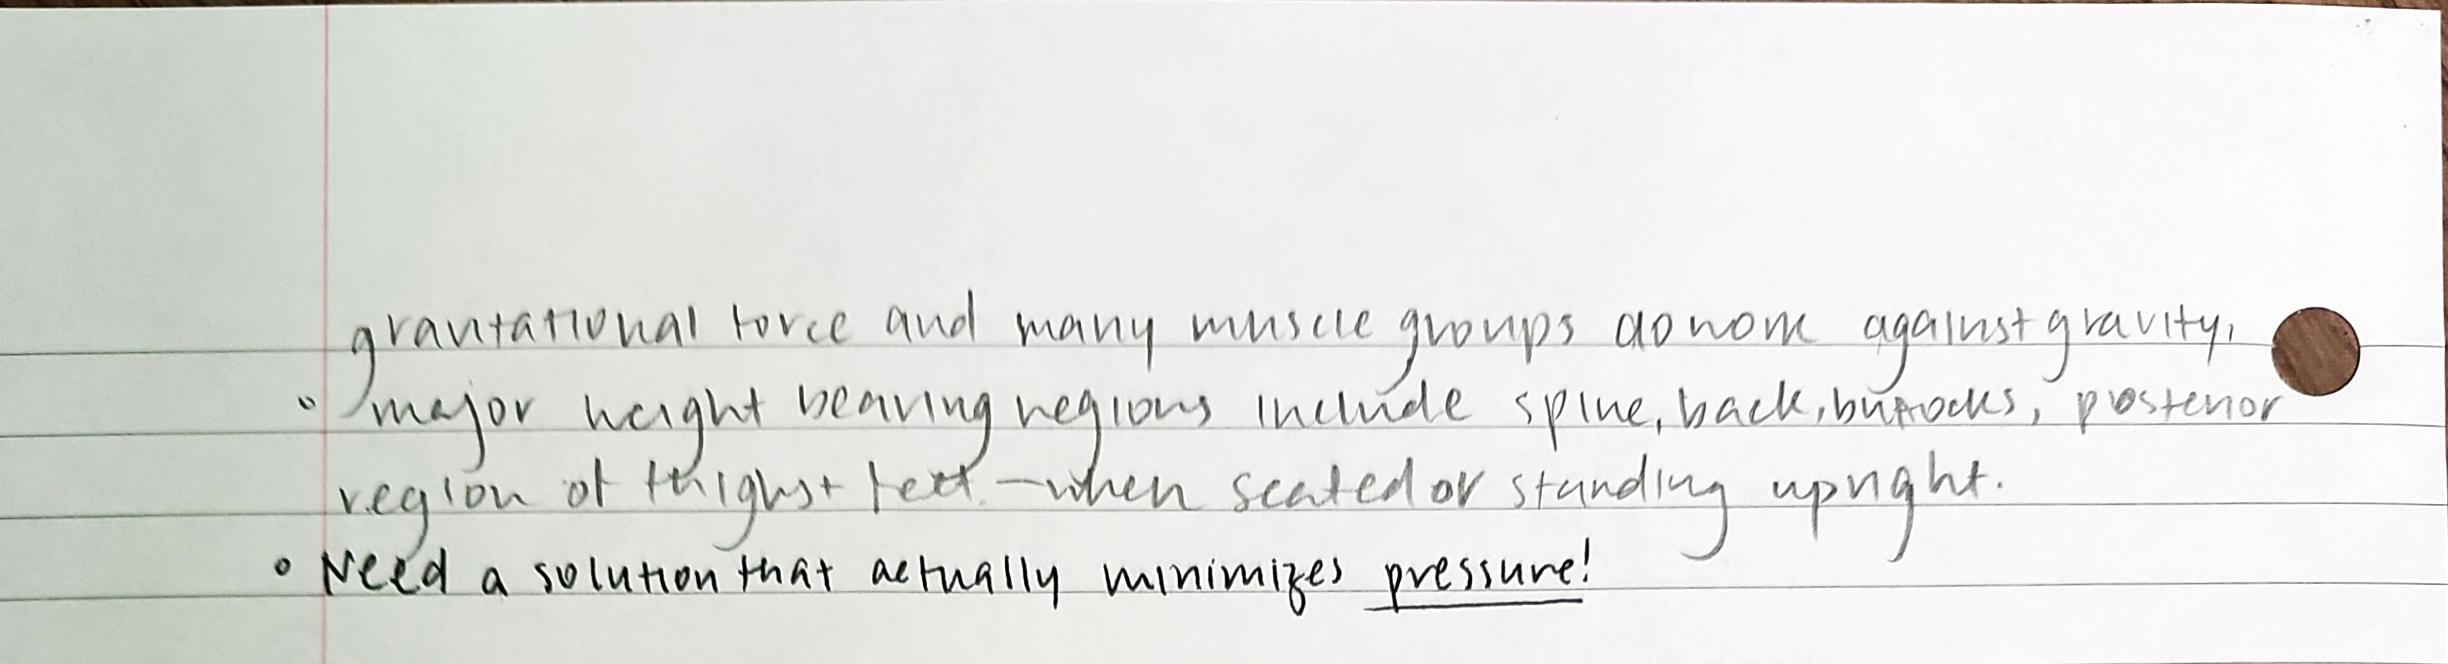
\includegraphics[width=1\linewidth]{second.png}
    \caption{Enter Caption}
    \label{fig:enter-label}
\end{figure}
\end{figure}
\end{document}
